\documentclass[twocolumn]{article}

\usepackage{graphicx}
\graphicspath{{../figs/}}
\usepackage[a4paper, margin=1.5cm, bottom=2.5cm]{geometry}
\usepackage{float}
\usepackage{subfig}
\usepackage{caption}
\usepackage{tabularx}
\usepackage{booktabs}
\usepackage{amsmath}
\usepackage{stfloats}
\usepackage{titlesec}
\usepackage{xcolor}
\definecolor{UIUC_orange}{HTML}{FF5F05}
\usepackage[colorlinks=true,
            linkcolor=UIUC_orange,
            urlcolor=UIUC_orange,
            citecolor=UIUC_orange]{hyperref}
\usepackage[
  backend=biber,
  style=numeric,          % numbered refs
  citestyle=numeric-comp, % [1-3] compression
  sorting=none            % order of citation
  ]{biblatex}
  \addbibresource{references.bib}
  
  \captionsetup[figure]{labelfont=bf, justification=justified, singlelinecheck=false}
  \captionsetup[subfloat]{labelfont=normalfont, justification=centering, singlelinecheck=false, farskip=4pt,captionskip=0pt}
  \captionsetup[figure]{belowskip=-14pt}
  \captionsetup[subfloat]{belowskip=-14pt}
  
  \captionsetup[table]{labelfont=bf, justification=justified, singlelinecheck=false, skip=2pt, farskip=0pt, captionskip=0pt, belowskip=0pt}
  
  
  \setlength{\columnsep}{0.5cm}
  
\makeatletter
\renewcommand\section{\@startsection{section}{1}{0pt}%
  {0.8ex plus 0.5ex minus 0.2ex}%
  {0.5ex}%
  {\normalfont\large\bfseries}}
\makeatother

\makeatletter
\renewcommand{\maketitle}{\bgroup\setlength{\parindent}{0pt}
\begin{flushleft}
  \Large\textbf{\@title}

  \vspace{0.2cm}

  \normalsize\@author \hfill \normalsize\@date

  \vspace{0.25cm}\hrule\vspace{0.25cm}
\end{flushleft}
\egroup}
\makeatother


\title{Rainfall-Soil Moisture Event Responses near Baton Rouge, Louisiana}
\author{%
  % Ali Haghighi\thanks{University of Tehran, \href{mailto:ahaghighi@ut.ac.ir}{ahaghighi@ut.ac.ir}}%
  % Afshin Ashrafzadeh\thanks{University of Tehran, \href{mailto:a.ashrafzadeh@ut.ac.ir}{a.ashrafzadeh@ut.ac.ir}}%
  Ali Haghighi \footnotesize{(ahaghighi@ut.ac.ir)}\normalsize, Afshin Ashrafzadeh
}
\date{\today}


\begin{document}

\twocolumn[
  \begin{@twocolumnfalse}
    \maketitle
  \end{@twocolumnfalse}
]

% \makeatletter
% \@thanks
% \makeatother

\section*{Introduction}

Rainfall controls soil moisture variability and drives hydrological processes from infiltration to contaminant transport. This study investigates event-scale rainfall-soil moisture interactions near Baton Rouge, Louisiana, during 2022-2024. We detect and analyze individual rainfall events, quantify associated soil moisture responses, and assess seasonal patterns in their magnitude and variability. The focus is on the change in soil moisture ($\Delta \theta$) as an indicator of infiltration dynamics.

Our results provide insight into how antecedent wetness and event precipitation shape soil moisture responses across seasons. Beyond immediate hydrological interpretation, this framework offers a basis for future extensions, including nitrate leaching and surface-subsurface contamination analysis, once nutrient datasets are integrated.

\textbf{Resources: }
Codes and processed data (spatially and temporally subsampled; easy-to-use CSV) are available on \href{https://github.com/Alioax/rainfall-soil-moisture/}{GitHub repository}. 
My personal website and other projects can be found at \href{https://ciarel.com}{Ciarel.com}.


\section*{Study Area and Data}

The analysis domain is a 25~$\times$~25~km box surrounding Baton Rouge, Louisiana (SW: 30.34,~-91.28; NE: 30.56,~-91.02), as shown in Fig.~\ref{fig:map}. This bounding box was chosen to capture regional hydroclimatic variability while maintaining a tractable spatial scale for event-based soil moisture analysis. Both precipitation and soil moisture datasets were subsetted spatially to this domain and temporally to the period 2022--2024.

\begin{figure}[!h]
  \centering
  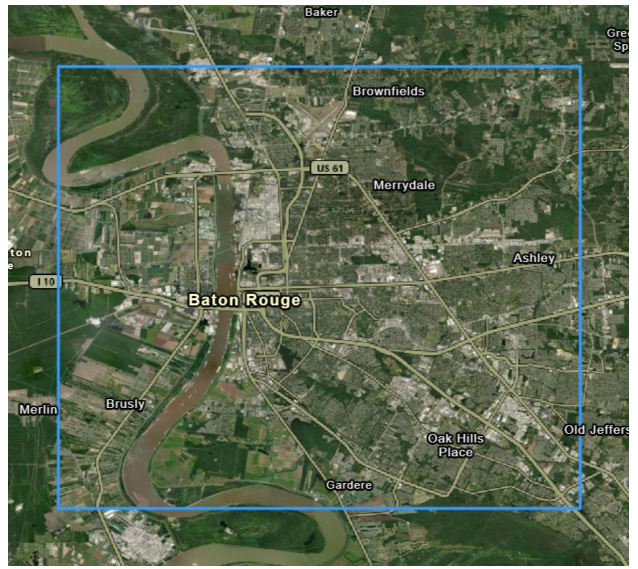
\includegraphics[width=0.95\columnwidth]{map}
  \caption{Study area near Baton Rouge, Louisiana. The analysis domain (25 $\times$ 25 km box) is outlined and overlain on regional context.}
  \label{fig:map}
\end{figure}

Soil moisture conditions were obtained from the NASA Soil Moisture Active Passive (SMAP) mission, using the Enhanced Level-3 Radiometer Global Daily product (9~km resolution), which provides surface soil moisture retrievals representative of the top $\sim$5~cm of soil \cite{smap}. Precipitation data were obtained from the Global Precipitation Measurement (GPM) mission's Integrated Multi-satellite Retrievals (IMERG) Final Run product, available at 0.1$^{\circ}$ spatial and daily temporal resolution \cite{imergdp}.

Together, SMAP and IMERG provide harmonized, global-scale, open-access satellite observations suitable for characterizing - moisture interactions in regions such as Baton Rouge, where high-frequency precipitation events and strong seasonal cycles affect vadose-zone hydrology.

\section*{Methods}

Rainfall events were defined from daily precipitation \(P_t\). A wet day is \(P_t \geq 1\) mm, and an event is a sequence of wet days that (i) starts after a dry day, and (ii) includes a burst of at least 5 mm on the first or second day. For an event with start \(s\) and end \(e\), total rainfall and duration are  

\[
R = \sum_{t=s}^{e} P_t, 
\qquad 
D = e - s + 1.
\]

Antecedent soil moisture is the mean of the three days before the event, but if these overlap with the previous event, we trim them. Let \(A\) denote this window and \(\theta_A\) its average. The post-event response window is  

\[
B = \big[s,\; \min(e+3,\; s_{\mathrm{next}}-1)\big],
\qquad 
\theta_{\max} = \max_{t \in B} \theta_t .
\]

The main metric is the soil moisture increment  
\[
\Delta \theta = \theta_{\max} - \theta_A .
\]

We also compute a nominal lag between antecedent and response times. However, we do not analyze it further because SMAP provides only surface soil moisture (\(\sim\)0--5 cm) at daily resolution. With no information from deeper layers, infiltration timing and true lags cannot be extracted reliably. If multi-depth soil measurements were available, lag analysis would be a valuable extension.  

\section*{Results}

\paragraph{Hydroclimatic context.}
Monthly precipitation and domain‐mean soil moisture (Fig.~\ref{fig:monthly_precip_sm}) track each other closely, with wetter months yielding higher soil moisture. Peaks occur at the end of winter and early spring, reflecting cumulative cool‐season rainfall and low evaporative demand.

\begin{figure}[!h]
  \centering
  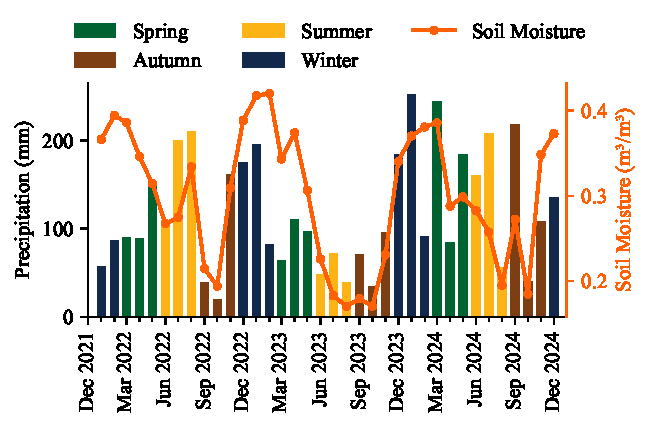
\includegraphics[width=1\columnwidth]{monthly_precip_sm}
  \caption{Monthly precipitation totals and averaged soil moisture from 2022-2024.}
  \label{fig:monthly_precip_sm}
\end{figure}

\paragraph{Rainfall events.}
Event characteristics are shown in Fig.~\ref{fig:rain_events}. The median event produced 25~mm over 2~days. High‐depth, long‐duration outliers (above the 75th percentile in both) occurred mainly in summer. Seasonal counts were Winter~31, Spring~31, Summer~29, and Autumn~23.

\begin{figure}[!h]
    \centering
    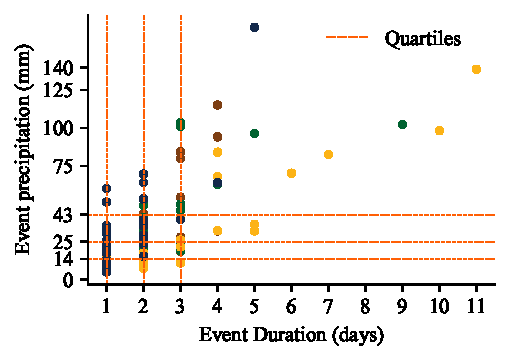
\includegraphics[width=0.75\columnwidth]{rain events}
    \caption{Event rainfall depth versus duration.}
    \label{fig:rain_events}
\end{figure}

\paragraph{Soil moisture responses.}

For each event, the soil moisture increment ($\Delta \theta$) was calculated. Fig.~\ref{fig:sample_events} illustrates sample events; smaller storms were sometimes missed by detection rules. Across all events (Fig.~\ref{fig:dt_events}, top), $\Delta \theta$ had a median of ~6\% and a maximum near 18\%. The left panel shows a clear saturation boundary: high antecedent moisture limits responses, while drier soils allow larger increases. Winter and spring cluster near saturation, consistent with Fig.~\ref{fig:monthly_precip_sm}, whereas summer-autumn span drier antecedent states with responses from 0-18\%. The right panel relates $\Delta \theta$ to precipitation: most events (0-50~mm) produced variable responses, indicating rainfall depth alone does not constrain soil moisture change.

\begin{figure}[!h]
    \centering
    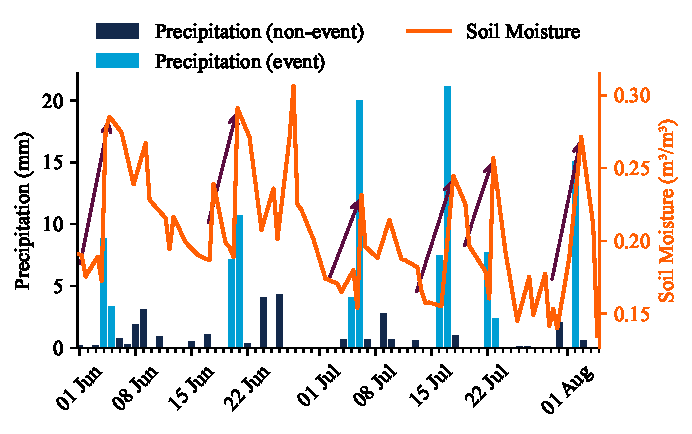
\includegraphics[width=\columnwidth]{sample events}
    \caption{Example rainfall event: daily precipitation and soil moisture response.}
    \label{fig:sample_events}
\end{figure}

\begin{figure}[!h]
    \centering
    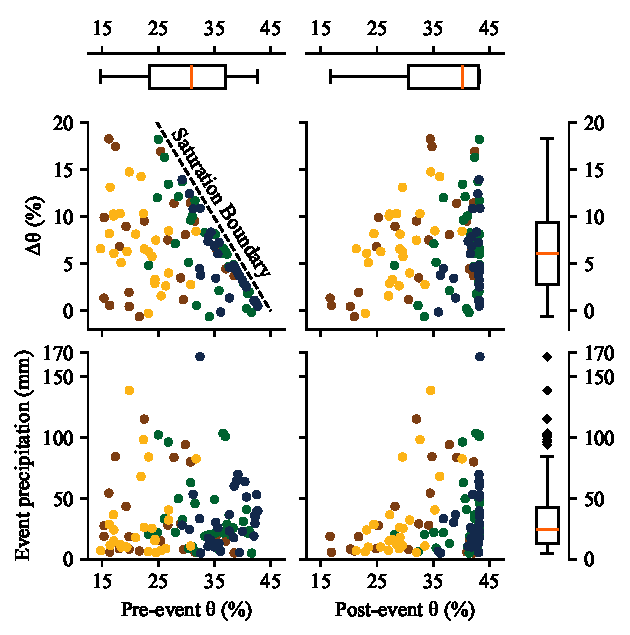
\includegraphics[width=\columnwidth]{dt events}
    \caption{Distribution of soil moisture change ($\Delta \theta$) versus antecedent soil moisture and event precipitation.}
    \label{fig:dt_events}
\end{figure}


\section*{Future Research}

Future research could potentially extend this event-based framework by coupling - moisture responses with a fully integrated water-heat-nitrate modeling approach, similar to recent work by \textcite{Fahs2025}. Such coupling would allow assessment of how storm-driven infiltration dynamics influence not only moisture but also temperature effects and nitrate mobilization in the vadose zone, thereby linking observed $\Delta \theta$ signatures to broader water-quality implications under seasonal variability.

\printbibliography

\end{document}
